\documentclass{article}


\usepackage{arxiv}

\usepackage[utf8]{inputenc} % allow utf-8 input
\usepackage[T1]{fontenc}    % use 8-bit T1 fonts
\usepackage{hyperref}       % hyperlinks
\usepackage{url}            % simple URL typesetting
\usepackage{booktabs}       % professional-quality tables
\usepackage{amsfonts}       % blackboard math symbols
\usepackage{nicefrac}       % compact symbols for 1/2, etc.
\usepackage{microtype}      % microtypography
\usepackage{lipsum}

\usepackage{times}
\usepackage{latexsym}

\usepackage{times}
\usepackage{url}
\usepackage{latexsym}

\usepackage{algorithm}
\usepackage{pifont}
\usepackage{tikz}
\usepackage{amsmath}
\usepackage{pgfplots}
\usepackage{balance}
\usepackage{multibib}

\usepackage{graphicx}
\usepackage{amssymb,amsmath,bm}
\usepackage{textcomp}
\usepackage{balance}

\usepackage{subfig}

\usepackage{mathtools}
\usepackage{booktabs}
\usepackage{array,dcolumn}


\setlength{\parskip}{-0.01cm}
\setlength{\parindent}{0em}
\linespread{0.91}

%\usepackage[]{algorithm2e}
\usepackage{algorithm,algpseudocode}
\usepackage{pgfplots}
\pgfplotsset{width=8cm,compat=1.8}
\usetikzlibrary{patterns}

\usetikzlibrary{shadows,arrows}
% Define the layers to draw the diagram
\pgfdeclarelayer{background}
\pgfdeclarelayer{foreground}
\pgfsetlayers{background,main,foreground}

% Define block styles  
\tikzstyle{materia}=[draw, fill=blue!20, text width=6.0em, text centered,
  minimum height=1.5em,drop shadow]
\tikzstyle{practica} = [materia, text width=8em, minimum width=10em,
  minimum height=3em, rounded corners, drop shadow]
\tikzstyle{texto} = [above, text width=6em, text centered]
\tikzstyle{linepart} = [draw, thick, color=black!50, -latex', dashed]
\tikzstyle{line} = [draw, thick, color=black!50, -latex']
\tikzstyle{ur}=[draw, text centered, minimum height=0.01em]
 
% Define distances for bordering
\newcommand{\blockdist}{2.3}
\newcommand{\edgedist}{2.5}

\newcommand{\practica}[2]{node (p#1) [practica]
  {Step #1\\{\scriptsize\textit{#2}}}}

% Draw background
\newcommand{\background}[5]{%
  \begin{pgfonlayer}{background}
    % Left-top corner of the background rectangle
    \path (#1.west |- #2.north)+(-0.5,0.5) node (a1) {};
    % Right-bottom corner of the background rectanle
    \path (#3.east |- #4.south)+(+0.5,-0.25) node (a2) {};
    % Draw the background
    \path[fill=yellow!20,rounded corners, draw=black!50, dashed]
      (a1) rectangle (a2);
    \path (a1.east |- a1.south)+(0.9,-0.28) node (u1)[texto]
      {\scriptsize\textit{#5}};
  \end{pgfonlayer}}

\setlength{\belowcaptionskip}{-10pt}

%\aclfinalcopy % Uncomment this line for the final submission
%\def\aclpaperid{***} %  Enter the acl Paper ID here

% To expand the titlebox for more authors, uncomment
% below and set accordingly.
% \addtolength\titlebox{.5in}    

\newcommand\BibTeX{B{\sc ib}\TeX}



\title{A Hybrid Framework for Topic Structure using Laughter Occurrences}


\author{
Sucheta Ghosh\\
        HITS gGmbH,\\
        Heidelberg,\\
        69117 Germany.
  %% \AND
  %% Coauthor \\
  %% Affiliation \\
  %% Address \\
  %% \texttt{email} \\
  %% \And
  %% Coauthor \\
  %% Affiliation \\
  %% Address \\
  %% \texttt{email} \\
  %% \And
  %% Coauthor \\
  %% Affiliation \\
  %% Address \\
  %% \texttt{email} \\
}

\begin{document}
\maketitle

\begin{abstract}
Conversational discourse coherence depends on both linguistic and paralinguistic phenomena. In this work we combine both paralinguistic and linguistic knowledge into a hybrid framework through a multi-level hierarchy. Thus it outputs the discourse-level topic structures. The laughter occurrences are used as paralinguistic information from the multiparty meeting transcripts of ICSI database. A clustering-based algorithm is proposed that chose the best topic-segment cluster from two independent, optimized clusters, namely, hierarchical agglomerative clustering and $K$-medoids. Then it is iteratively hybridized with an existing lexical cohesion based Bayesian topic segmentation framework. The hybrid approach improves the performance of both of the stand-alone approaches. This leads to the brief study of interactions between topic structures with discourse relational structure. This training-free topic structuring approach can be applicable to online understanding of spoken dialogs.
\end{abstract}


% keywords can be removed
\keywords{topic structure \and Spoken dialog \and paralinguistics}


\section{Introduction}
Topic structures are basically a type of discourse structure. There exists many methods for topic segmentation those use semantic, lexical and referential similarity or, more recently, the language models \cite{hearst-97,elhadad-99,utiyama-01,galley-03,malioutov-06,eisenstein-08}. An automated topic segmentation tool splits a discourse into a linear sequence of topics such as the geography of a country, followed by its history, demographics, economy, legal structures, etc.; this segmentation is usually done on a sentence-by-sentence basis, with segments not assumed to overlap \cite{webber-12}. %Additionally, the term discourse segmentation is used to refer to any segmentation of a discourse into a ``high-level'' linear structure\cite{jurafsky-09}. 
In this work the whole process utilizes a stage-by-stage procedure like it is devised by \cite{grosz-86}. Thereby we achieve a discourse level topic structure, beyond the sentence level structure. In our case, segmentations with overlaps do not have much relevance because our primary level segmentation is done on the basis of shared laughter occurrences in meeting dialog; during those laughter turns there exists out-of-topic and fragmented comments. So we acquire a high level hybrid structure of topic, that combines the local and global levels of segmentation through a multi-level hierarchy of linear segmentations. %The whole process of this work largely follows the work of \cite{grosz-86}, that also defines a stage-by-stage framework. Here we do not acquire any overlapping segmentation, it is a hierarchy of coarse and fine-grained linear segmentation. 
%Multiparty conversation segmentation aims at the coherent, non-overlapping splits of conversation transcripts. This segmentation enables us to understand the discourse and topic structure of the conversation\cite{ivana2003}. The conversation segmentation can be linear or hierarchical. The linear segmentation attempts to find discourse, topic boundaries within a text without any concern of their underlying structure, whereas a hierarchical segmentation not only locates the local discourse or subtopics, but also tries to organize them into a meaningful hierarchy. We present here a two-stage segmentation technique relying on a hierarchy of two level linear segmentation. 

%In this work, we propose a framework that works in a hierarchy of two levels for natural conversation. On the first level, it uses paralinguistic information to segment the conversation according to the change in topics; in the next level, we use these primary linear segments iteratively to find the fine grained topic structure using an existing unsupervised lexical topic segmentation tool. Our proposed multi-stage hybrid technique basically combines the local and global levels of segmentation.

%The whole process largely follows the work of \cite{grosz-86}. Like them, we also follow a three stage process: 1. at the first stage we acquire the discourse segments on the basis of laughter occurrences, 2. then instead of a focus space stack we use an iterative process that works in an incremental manner, which processes the current acquired segments in each step with respect to the previous segment splits, thus it does not wait or depend on the acquisition of the whole data of the conversation. and 3. through each iteration the third-party lexical topic segmentation tool makes fine-grained segmentation on the basis of the prominence of the topics. This way the hybrid method improves the performance of the stand-alone approaches. In addition to that, it offers a higher-level structure than a plain global level topic segmentation structure.

%Like any other discourse structure, the segmentation can be accomplished either at a fine or coarse-level. In contrast to the fine-grained discourse processing methods, the coarse-level method of analysis does not go into details of the inter-clausal or inter-sentential phenomena; it considers only the chunks of the turn utterances as a meaningful segment. It is seen that in many of the discourse processing tasks like dialog generation, the level of analysis plays a very important role. %We may need to conceive the shift of the fine and coarse-level discourse to understand the shift of the focus of comprehension in a conversation. It is also seen that the coarse level segmentation of a full document or conversation is an essential step to process the fine-grained discourse \cite{hearst-97}. 


%%Several previous works use syntactic \cite{bestgen2000}, lexical knowledge \cite{stokes2002} of the language of the meeting or broadcast news transcripts, some others also exploit the other linguistic features like prosody\cite{nakatani1995}, some used pure machine learning with hidden Markov model to learn topic segments from the transcripts\cite{sherman2008}. %Although it was always evident to the community that in the conversational discourse segmentation the paralinguistic aspects are also important to the linguistic aspects \cite{holt-10,quek2000}, only a few works used paralinguistic information with linguistic information. 
%%This is subject to transcription quality, syntax-errors and language resource specificity. 
%%%It is also hard to acquire an accurate measurement of prosodic features like pitch.
%%In addition to linguistic knowledge, paralinguistic features are also used in conversation. One needs both kinds of information for a perfect comprehension. However, due to the following issues the integration of paralinguistic knowledge is a challenging task: (1) need to align two different kinds of informations in a framework. (2) need of annotated good amount of data with paralinguistic information. (3) need to acquire an accurate measurement of prosodic features like pitch. (4) It also becomes hard to execute the same techniques over various languages, especially while we are dealing with low resource languages. On the other hand, paralinguistic informations do not depend on the grammar or syntax of languages; when we solely rely on the linguistic features, and we discard the paralinguistic information, thus we miss the crucial information important to understand the structure of coherence. Besides, the paralinguistic information alone does not constitute the whole structure of coherence. Therefore, we propose a hybrid framework that makes use of both paralinguistic and lexical information in a two-stage hierarchy.

%There exists numerous techniques to segment a conversation using various supervised and unsupervised discourse, topic segmentation methods. These methods are generally comprised of machine learning processes and lexical and/grammatical knowledge. On the other hand, we note that there exists several works in the area of psychology those conclude that paralinguistic cues like laughter are very helpful features in discourse, topic segmentation\cite{holt-10,quek2000}. 

In this work, we propose a training-free framework for conversation segmentation incorporating the psychological evidences of coherence in conversation segmentation. According to the literatures of psychology, shared vocalized laughter in a conversation invariably denotes the change of topic, the vice versa is not necessarily true, that is, in a conversation sometimes the topic changes occur without any occurrence of laughter \cite{holt-10}. Therefore, if we are able to locate the shared laughter occurrences in a conversation, it will veritably indicate the segments with same topics. %First we exploit this observation to achieve a basic conversation segmentation using 2-way-parallel processed clustering technique. We attempt also to optimize the performance of both of these clustering techniques. 
To achieve this, we acquire the laughter occurrences from the annotations of database. Then we cluster the laughter occurrences. Based on the number of cluster membership the shared laughter occurrences are identified. The shared laughter occurrences determine the segment boundaries. To ensure the robustness of optimization two clustering techniques are applied independently: agglomerative hierarchical clustering and $K$-medoids. These techniques were optimized and integrated to achieve the best performance, namely, fixed boundary clumping for hierarchical clustering and iterative optimization for $K$-medoids. 
Then we hybridize this basic (clustering based) segmentation with a lexical cohesion based Bayesian text segmentation method \cite{eisenstein-08}. The resultant hybrid method performs better than the stand-alone approaches. The approach is fit for online setup.%It is possible to use the same hybrid algorithm with other similar kind of linear segmentation technique to achieve another hybrid form of linear segmentation. 

The goal of this work is not merely to improve the state of the art performance combining multiple methods. This is to show that the linguistic and paralinguistic information are both useful to achieve a conversational topic discourse. Also, we conduct a brief study of interaction between topic structure and the discourse relational structure. %%Additionally, we make a comparative study between our proposed hybrid topic structure and a discourse relational structure. This study hints that most of the cases the topic-in-focus density is high in proximities of the discourse connective. %It addresses a critical problem which is the information alignment problem when using all possible kinds of informations. It is possible to use the same hybrid algorithm with other kind of segmentation technique to achieve another hybrid form of segmentation.

\subsection{Related Works}\label{sec:relwrk}
%A large number of discourse and topic segmentation techniques have been developed for more than two decades of time. 
%\cite{hirschberg-96,hearst-97,elhadad-99,shriberg-00,utiyama-01,galley-03,malioutov-06,eisenstein-08,niekrasz-09,niekrasz-10}. Still there is the need for this task in various areas of research related to human languages technologies. The immediate application is changing according to the current needs and data specifications; as well the proposed frameworks are performing better than the previously existing frameworks. Therefore most of the mentioned works are still largely used or cited as baselines.
%This is yet an open problem for many language technologies. 

A significant number of segmentation techniques are based on lexical cohesion \cite{hearst-97,elhadad-99,utiyama-01,galley-03,malioutov-06,eisenstein-08}. %TODO:[need to check the citation style]. 
\cite{halliday-76}'s seminal work states about two main types of cohesion, namely (1) grammatical, which is based on structural content, and (2) lexical, which is based on lexical content and background knowledge. There exists some grammatical cohesion based segmentation techniques \cite{giora1983,bestgen2000,taboada-09}. %We prefer not to use the grammatical information to achieve better adaptability and applicability of the method across many languages. So in this work, we choose a third-party tool for our framework that uses lexical cohesion in the Bayesian context, thus it makes it easy to apply for many languages. This lexical cohesion based tool is basically developed using monologue text corpus, but it can be used for the user transcripts as well.%The lexical cohesion is largely used for this specific task of text segmentation \cite{hearst-97,elhadad-99,utiyama-01,galley-03,malioutov-06,eisenstein-08}[need to check the citation style]. 
%
While most of the prominent works in the conversational segmentation are based on lexical cohesion, the cue word or phrase based segmentation techniques are also prevalent. The theory by \cite{grosz-77} proposes the usage of some cue word or phrase as discourse markers. %It is also proved to be very beneficial for the task \cite{grosz-77}. The choices of connectives are generally task or corpus-statistics specific. In this work, the over-mentioned third-party tool also uses cue word based approach using corpus statistics\cite{eisenstein-08}.

There exists some linear conversation segmentation techniques \cite{hearst-97,kaufman1999,eisenstein-08}, but there also exists some works on the hierarchical segmentation \cite{eisenstein-09,simon2015}. In both the cases the methods based on lexical cohesion and Bayesian learning are most successful.%An algorithm is developed by Eisenstein for the hierarchical segmentation using Bayesian learning based lexical cohesion\cite{eisenstein-09}. %Like most of the prominent works this third party tool extracts fine-grain segmentation.%TO ADD MORE DETAILS

The task of discourse segmentation started in a supervised setup with written texts using cue words or cue phrase discourse marker \cite{grosz-77,litman-93,elsner-08}. The problem is that these studies are constrained with respect to the important factors like available resources, dealing with the problems of spoken language wide variability, dealing with the multi-lingual setup.
%
%Although most these prominent methods primarily adopt supervised techniques, for conversations or written texts, there exists several successful training-free approaches of segmentation techniques that overcome many problems faced by the former trained frameworks, for example obviously it may not depend on the availability of resources or it can partly depend on. 

\cite{hearst-97} defined subtopic groupings for science-news article paragraphs into some classes, which evolved into present day templates that can be filled with proper values. This work called TextTiling, is basically a cohesion based approach. The work of \cite{choi-00} used a divisive clustering algorithm to linearly segment the text. In the unsupervised model of \cite{galley-03}, inference is performed by selecting segmentation points at the local maxima of the cohesion function. \cite{malioutov-06} optimized a normalized minimum-cut criteria based on a variation of the cosine similarity between sentences.

There also exists a series of notable works those use Bayesian approach to linearly segment the topic. As we know that Bayesian inference is fit for dynamic analysis of sequential data, and also it is easier to incorporate additional features or resources like language model with a Bayesian framework. The work of \cite{eisenstein-08} showed an way of unsupervised topic segmentation using Bayesian approach , whereas the work of  \cite{utiyama-01} was a special case of Bayesian learning; an alternative Bayesian approach was also proposed by \cite{purver-06}.

Among all the other existing approaches the lexical cohesion based unsupervised Bayesian approach by \cite{eisenstein-08} is one of the important frameworks. In their work the authors show that the lexical cohesion can be placed in a Bayesian context by modeling the words in each topic segment as it draws from a multinomial language model associated with the segment; maximizing the observation likelihood in such a model it yields a lexically-cohesive automatic segmentation \cite{eisenstein-08}. The Bayesian framework provides a principled way to incorporate additional features such as cue phrases, which is a powerful indicator of discourse structure in the unsupervised segmentation frameworks.  %This work is quite popular in the community even if it is some years old. 
This model still offers consistent improvements over an array of state-of-the-art systems on both text and speech datasets. Therefore we choose the work as one of our baselines. %In the next step we propose a hybrid approach that uses this existing approach and our proposed clustering based approach in iterations. It is also possible to replace this standalone third-party framework with other segmentation framework depending on the performance and task.

%There is a division between linear and hierarchical segmentation tasks. %In some cases the document is pre-structured, for example the bio-medical texts are \emph{functionally} pre-segmented from its generation viz. Background, Method, Result, Discussion. Automatic determination of both of the pre-structured and linearly segmented discourse structure, is not a trivial task. Moreover, linear segmentation of raw text can be useful for the hierarchical segmentation task. In fact our proposed algorithm in this paper works in a hierarchy on a primary linear segmentation and produce better results than stand-alone setups. There exists several other interesting works for example Eisenstein developed an algorithm for hierarchical segmentation using Bayesian learning based lexical cohesion\cite{eisenstein-09}.

We have described the topic segmentation methods for written texts, which is either a well structured document or a semi-structured or unstructured transcribed conversation. There also exist seminal works on spoken discourses: both of \cite{hirschberg-96} and \cite{niekrasz-09} use the prosodic phrases, the latter used linguistic features and the former used low level paralinguistic, prosodic features like pitch, duration. The accurate extraction of low-level prosodic features is still a challenging area. 

%Besides, the solo text based and solo speech based segmentation methods there exists a few works which use both text and speech based features \cite{liu2009}. They used the intonation patterns, cue words and prosodic units as features for the method based on statistics. It is to be mentioned here that in this work we emphasize on not only to use all possible kind of data but also to find a possibility to align all the data through stages, not merely using as a bag of features like we do for any general classification problem. % TO GIVE MORE STUFFS ABOUT

In this work we also aim at incorporating the knowledge from cognitive psychology, by the means of human laugh occurrences. Prior works of \cite{holt-10}, \cite{bonin-12} already stated that there is an evident link between the topic change and laughter in human-human discourses. Studies also report that the voiced laughter generates positive affect \cite{bachorowski-01}; the mirthful laughter activities have been suggested as modifiers of neuroendocrine hormones involved in the classical stress response \cite{berk-89}, and the stress has a negative effect on human attention \cite{jensen-98}. In the meetings, people generally use laughter as a de-stressing activity and then move on to a new discourse or topic. It may also be possible that a meeting does not contain any laughter situation, this study does not cover that situation, it only covers the natural human conversations with laughter.

%\subsection{Usage of Laughter in Conversation Segmentation}\label{sec:mot}
\subsection{Motivation: hybrid segmentation of conversation using laughter}\label{sec:mot}
Spoken language comprehension does not depend only on the text or the words. The cognitive model of language comprehension by \cite{bower-85} states about a step-by-step comprehension process. On the first steps the words are recognized; on the subsequent steps the prosody and gestures are involved, thus finally the whole matters are comprehended through the extraction of features and pattern recognition. There exists many paralinguistic features those are actively involved in this process of comprehension.  Among all paralinguistic features, laughter surely plays an important role, that we already discussed in \ref{sec:relwrk} citing the several works, and also there we mentioned about our preference for the stage by stage processing for various kinds of informations. %there are many kinds of laughter as we have already seen from the related works. Among all the kinds of laughter the shared laughter in a conversation is connected with the topic changes in a conversation \cite{holt-10}. 

It is interesting to conduct a study of interaction of the topic structure and any other discourse structures, namely discourse relational structure. On the other hand, the real-time classification in spoken language understanding seeks those approaches, which can also be used as online framework. In this case, we do not wait until all the data is captured before starting the online process of understanding. The frameworks internally process data, segment by segment with no dependency on the future. Thus if we can acquire the transcripts through an online Automatic Speech Recognizer \cite{kaldionline16} and also if we be able to achieve laugh occurrences\cite{salamin13,schuller13,ghosh16}, then we are able to acquire this topic structure online. %Therefore a proper segmentation strategy plays an important role on the success of the online algorithm. Therefore we deliberately choose an approach that is a fit for working as a real-time system that can work incrementally, hybridizing coarse and fine grained segmentations in hierarchy. 

%Therefore it is evident that occurrence of any kinds of laugh does not necessarily segments the data in a comprehensive manner, only shared laughter is connected to the topic change in a multiparty conversation, but the vice versa is not true i.e. topic changes in a conversation can also occur without any occurrence of shared laughter \cite{holt-10}. Therefore it is possible to use the shared laughter as a tool to capture the topic or discourse change in a gross scale. Thus it is possible to achieve a coarse-level conversation segmentation though the determination of the shared laughter occurrences in a conversation. We also know from the work of Hearst (1997) that the coarse-level meaningful segmentation a sufficiently helpful step for many language or conversation comprehension tasks \cite{hearst-97}.

\subsection{Our Contribution}\label{sec:cont} 
In this work, we present a framework that follows a cascaded process that hybridizes two standalone processes in a hierarchy: at the first level we segment a conversation using paralinguistic information laughter, then at the next level, we include a third party tool for topic segmentation of the text, subjected to the primary paralinguistic segmentation. We observe a significant improvement of result of this hybrid framework in comparison to the standalone techniques. The goal of this hybridization is not merely to improve the baseline; through this work we propose a framework that not only works along with the cognitive model of human comprehension \cite{bower-85}, but also it improves the baseline. Thus there remains the possibility to use the same framework in different context of spoken language comprehension. Additionally, here we study on the interaction between the topic and discourse relational structures. 

%The iterative algorithm that hybridizes two standalone processes is designed in such a way that it includes and use data without any dependency on the future. It considers on the current segment and also the previously acquired segments at one step of iteration, without any consideration about the future segments. Therefore this process is perfectly able to be used in a real-time spoken language understanding scenario. %This is a training-free approach. 
%The proposed method is applicable to any multiparty natural conversation in any languages, given we change the third party tool. This approach can be used with incremental learning in a range of application areas. For example, the systems like the meeting assistant system like CALO \cite{tur2010} can be developed and improvised with the proposed framework, and this is a complete fit for any real-time system. It may also facilitate text structuring and summarization task in an online setup. 
%in the style of a completely automatic framework by Salton et al (1997) \cite{salton1997}, 
%
%Holt (2010) studied that shared laughter in a meeting veritably denotes the topic changes in conversation, solo laughter does not necessarily follow that rule, also topic changes may happen without any occurrence of shared laughter \cite{holt-10}. This observation is used in this work to segment a conversational discourse using meeting transcripts. We use laugh occurrences to achieve coherent conversational segmentation. As a next step, we use this coherent segmentation to iteratively run a lexical cohesion based fine-grained topic segmentation algorithm, to achieve a hybrid hierarchical segmentation. 
%
%We consider only the vocalized laughter turn indices, which is a kind of anchor points in a conversation as the inputs. The laugh occurrences in the data are marked by the annotators. %To our best of knowledge, no framework is designed till date that segments a full meeting conversation using only laughter turn index information. We attempt to design a simple and comprehensive framework. %We call this minimal framework as cognitively intuitive because it is possible for a human being to trace back in the memory the coherence structure of a meeting following all the anchor points of laughter moments (for example, specific jokes related to a topic in discussion). 

%To achieve this multi-stage hierarchical segmentation of the whole conversational discourse, we primarily use the two kinds of clustering techniques: the agglomerative and the $K$-medoids clustering techniques, then we optimize the primary segmentation with boundary clumping for the former case and iterative optimization technique for the latter. We run these two techniques in parallel with the same input, and then we choose the best performing one for each of the conversation. At the next level, we hybridize this clustering based framework with a well-performing lexical cohesion based Bayesian text segmentation framework. We see that the hybrid framework out performs the stand-alone approaches. 

%In this paper, we describe the related works of this research area in the subsection \ref{sec:relwrk}, in the subsection \ref{sec:mot} we emphasize the motivation of the work, then we summarize our contribution in the next subsection \ref{sec:cont}. Further, we illustrate our methods: first about the stand-alone method in the section \ref{sec:hybseg} that describes the human laugh occurrence based on clustering methods. We used two kinds of clustering methods for optimization of segmentation decision: one follows agglomerative clustering in the section \ref{sec:hclus}, The optimization of this segmentation is described in the section \ref{sec:opthclus}; the other clustering segmentation technique is based on $K$-medoids, is depicted in the section \ref{sec:kmclus}, its optimization technique is noted in the section \ref{sec:optkmclus}. Next to this, we elaborate on the hybridization of this best performing clustering based segmentation and the state-of-the-art lexical cohesion based Bayesian text segmentation in the section \ref{sec:hyb}. In the following sections we explain the experimental setup in the section \ref{sec:expt}, where we also provide the details on our data, metrics and the experimental set-up, then subsequently we also discuss about the results. Finally, we conclude with a concise description of the whole work in the section \ref{sec:concl}.

%\subsection{Intro for Laughter Detection}

\section{Laughter based Hybrid Segmentation of Conversation}\label{sec:hybseg}
The two simultaneous way of processes and a four-step approach is followed to achieve this hybrid segmentation of the conversational discourse. We depict all four stages and two simultaneous processes in the Figure \ref{fig:proc}.

First, an initial segmentation is achieved using agglomerative hierarchical clustering technique; we use clustering because it is a flexible technique, in worst case this is better than any chance experiment, specifically the hierarchical clustering produces deterministic results and stores much information in its structure.%; then the optimization of the clustered segmentation using the process of fixed boundary clumping technique. %We follow \cite{niekrasz-10} for this clumping task., we also follow an iterative sliding window technique to optimize the boundaries of the segmentation. We use the metrics iteratively to optimize the boundaries.

We use two kinds of clustering to make the decision robust. In parallel to the hierarchical clustering, we employ another segmentation technique based on $K$-medoids clustering using the same input of the agglomerative clustering technique. $K$-medoids clustering is a flat clustering technique like $K$-means clustering. $K$-means is a classical robust partitioning technique of clustering that clusters the data set of n objects into $K$ clusters if $K$ known \emph{a priori}. The $K$-medoids algorithm is a clustering algorithm related to the $K$-means algorithm and the median-shift algorithm \cite{shapira-09}. Median-shift is a mode seeking algorithm that relies on computing the median of local neighborhoods, instead of the mean.

In contrast to the $K$-means algorithm, $K$-medoids chooses datapoints as centers, and in case of $K$-means the distances between the centroids of cluster set are calculated using $L2$-norms whereas in case of the $K$-medoids it uses $L1$-norms to calculate the distance between the medoids. The details of the method is given in the next section \ref{sec:kmclus}. Likewise the $K$-means, The $K$-medoids algorithm algorithm uses an iterative refinement technique for the optimization of performances.
%
As a second step, we optimize the primary segmentation of the agglomerative clustering through a fixed boundary clumping following \cite{niekrasz-10}, and as well, we optimize the primary segmentation of the K-medoids clustering through an iterative process.
%
In the third step, we choose the best performing segmentation between the agglomerative and $K$-medoids clustering. 
%
Finally, in the fourth step we hybridize this clustering based framework with the lexical cohesion based Bayesian text segmentation framework. Then we obtain the output of segmented conversation by means of the clustered turn-indices.  

\vspace{-0.01em}
%\begin{center}
\begin{figure}
%%%%\begin{tikzpicture}[scale=0.7,transform shape]
%%%%
%%%%  % Draw diagram elements
%%%%  \path \etape{1}{Raw signal};
%%%%
%%%%  \path (p1.south)+(0.0,-1.5) \etape{2}{Pre-1};
%%%%  \path (p2.south)+(0.0,-1.0) \etape{3}{Pre-2};
%%%%
%%%%  \path (p3.south)+(0.0,-1.5) \etape{4}{Feature extract};
%%%%  \path (p4.south)+(0.0,-1.0) \etape{5}{Model fitting};
%%%%
%%%%  \path (p5.south)+(-3.0,-2.0) \etape{6}{training};
%%%%  \path (p5.south)+(3.0,-2.0) \etape{7}{testing};
%%%%  \node [below=of p5] (p6-7) {};
%%%%
%%%%  \path (p6.south)+(0.0,-2.0) \etape{8}{normal};
%%%%  \path (p7.south)+(0.0,-2.0) \etape{9}{abnormal};
%%%%  \node [below=of p6-7] (p8-9) {};
%%%%
%%%%  % Draw arrows between elements
%%%%  \path [line] (p1.south) -- node [above] {} (p2);
%%%%  \path [line] (p2.south) -- node [above] {} (p3);
%%%%  \path [line] (p3.south) -- node [above] {} (p4);
%%%%  \path [line] (p4.south) -- node [above] {} (p5);
%%%%
%%%%  \background{p2}{p2}{p3}{p3}{bk1}
%%%%  \background{p4}{p4}{p5}{p5}{bk2}
%%%%  \background{p6}{p6}{p7}{p7}{bk3}
%%%%
%%%%  \path [line] (p5.south) -- node [above] {} (bk3-n);
%%%%  \path [line] (bk3-s) -- node [above] {} (p8);
%%%%  \path [line] (bk3-s) -- node [above] {} (p9);
%%%%  \path (bk1-w)+(+6.0,0) node (ur1)[ur] {};
%%%%  \path (bk2-w)+(+6.0,0) node (ur2)[ur] {};
%%%%  \path (bk3-w)+(+3.0,0) node (ur3)[ur] {};
%%%%  \transreceptor{bk1-w}{pre processing}{ur1};
%%%%  \transreceptor{bk2-w}{Feature selection}{ur2};
%%%%  \transreceptor{bk3-w}{classification}{ur3};
%%%%\end{tikzpicture}
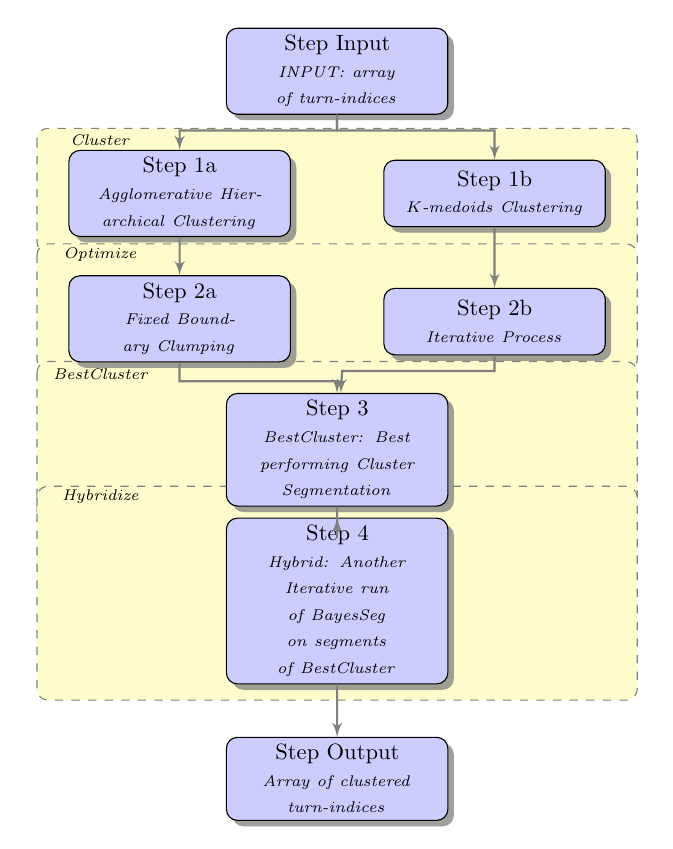
\begin{tikzpicture}[scale=0.80,transform shape]
 
  % Draw diagram elements
 %\path \practica {1}{Diferencias en componentes electr\'onicos};
%  \path (p1.south)+(0.0,-1.0) \practica{2}{Serie de Fourier};
%  \path (p2.south)+(-2.5,-1.5) \practica{3}{Antena para HF};
%  \path (p3.south)+(0.0,-1.0) \practica{5}{Medidor de SWR};
%  \path (p3.south)+(5.0,-1.0) \practica{4}{Amplificador para HF};
%
  %\path (p4.south)+(-2.5,-1.5) \practica{6}{Oscilador de RF};
  \path \practica {Input}{INPUT: array of turn-indices};
  \path (pInput.south)+(-2.5,-1.25) \practica{1a}{Agglomerative Hierarchical Clustering};
  \path (pInput.south)+(2.5,-1.25) \practica{1b}{$K$-medoids Clustering};
  %\path (p1b.east)+(+5.5,0) node (ur1)[ur] {};

  \path (p1a.south)+(0.0,-1.3) \practica{2a}{Fixed Boundary Clumping};
  \path (p1b.south)+(0.0,-1.5) \practica{2b}{Iterative Process};
%    \path (p2b.east)+(+5.5,0) node (ur4)[ur] {};
  \path (p2b.south)+(-2.5,-1.5) \practica{3}{BestCluster: Best performing Cluster Segmentation};
 \path (p3.south)+(0.0,-1.5) \practica{4}{Hybrid: Another Iterative run of BayesSeg on segments of BestCluster};
 \path (p4.south)+(0.0,-1.5) \practica{Output}{Array of clustered turn-indices}; 
%  \path (p17.south)+(0.0,-1.5) \practica{18}{Gu\'ias de ondas};
     
  % Draw arrows between elements
%  \path [line] (p1.south) -- node [above] {} (p2);

%  \path [line] (p2.south) -- +(0.0,-0.5) -- +(-2.5,-0.5)
%    -- node [above, midway] {} (p3);
%\path [line] (p3.south) -- node [above] {} (p5) ;
     
%  \path [line] (p2.south) -- +(0.0,-0.5) -- +(+2.5,-0.5)
%    -- node [above, midway] {} (p4);
%  \path [linepart] (p3.east) -- +(+0.5,-0.0) -- +(+0.5,-1.75)
%    -- node [left, midway] {} (p4);
%  \path [linepart] (p3.east) -- +(+0.5,-0.0) -- +(+0.5,-1.75)
%    -- node [left, midway] {} (p4);

%  \path [line] (p4.south) -- +(0.0,-0.5) -- +(-2.5,-0.5)
%    -- node [above, midway] {} (p6);
%  \path [line] (p5.south) -- +(0.0,-0.5) -- +(+2.5,-0.5)
%    -- node [above, midway] {} (p6);     
%  \path [linepart] (p2.east) -- +(2.75,0.0) -- +(2.75,-5.85)
%    -- node [right] {} (p6);
  \path [line] (pInput.south) -- +(0.0,-0.25) -- +(-2.5,-0.25)
    -- node [above, midway] {} (p1a);
  \path [line] (pInput.south) -- +(0.0,-0.25) -- +(+2.5,-0.25)
    -- node [above, midway] {} (p1b);
%  \path [linepart] (p7.east) -- node [left] {} (p8);
%  \transreceptor{p8}{AM banda 40m}{ur1}

  \path [line] (p1a.south) -- node [above] {} (p2a) ;
  \path [line] (p1b.south) -- node [above] {} (p2b) ;
%  \path [linepart] (p9.east) -- node [left] {} (p10);
%  \transreceptor{p10}{CW}{ur2}
%  \path [line] (p9.south) -- node [above] {} (p11) ;
%  \path [line] (p10.south) -- node [above] {} (p12) ;
%  \path [linepart] (p11.east) -- node [left] {} (p12);
%  \transreceptor{p12}{FDMDV}{ur3}

%  \path [line] (p11.south) -- node [above] {} (p13) ;
%  \path [line] (p12.south) -- node [above] {} (p14) ;
%  \path [linepart] (p13.east) -- node [left] {} (p14);   
%  \transreceptor{p14}{SSTV}{ur4}

  \path [line] (p2b.south) -- +(0.0,-0.25) -- +(-2.42,-0.25)
    -- node [above, midway] {} (p3);
  \path [line] (p2a.south) -- +(0.0,-0.3) -- +(+2.5,-0.3)
    -- node [above, midway] {} (p3);
    
  \path [line] (p3.south) -- +(0.0,-0.5) -- node [above] {} (p4) ;     
  \path [line] (p4.south) -- node [above] {} (pOutput) ;
%  \path [line] (p17.south) -- node [above] {} (p18) ;
   
%  \background{p7}{p1}{p8}{p2}{I}
%  \background{p7}{p3}{p8}{p5}{II}
  \background{p1a}{p1b}{p1b}{p1a}{Cluster}
%  \background{p7}{p9}{p8}{p10}{IV}
%  \background{p7}{p11}{p8}{p12}{V}
  \background{p1a}{p2a}{p1b}{p2b}{Optimize}
  \background{p1a}{p3}{p1b}{p3}{BestCluster}
 \background{p1a}{p4}{p1b}{p4}{Hybridize}
%  \background{p7}{p18}{p8}{p18}{IX}
\end{tikzpicture}
\caption{\footnotesize The diagram of basic processes of the whole hybrid framework}\label{fig:proc}
 \end{figure} 
 %\end{center}
 \vspace{-0.01em}

\subsection{Segmentation using Agglomerative Clustering}\label{sec:hclus}
This work uses multiparty meeting conversations. Each document is defined as a linear sequence of turns occurring from many participants. Each document is a global discourse, whereas we aim at segmenting this whole document into linear chunks, that is for a M-length sequence of turns $\langle t_1, t_2 \cdots t_M \rangle$  in a global discourse, minimal local discourse boundaries are $\langle [0,t_1\},\{t_1,t_2\}, \cdots \{t_{M-1}t_M\}, \{t_M, D]\rangle$, $0$: the starting point, $D$: ending point. A potential segmentation $X$ can be defined as a collection of non-overlapping subsequences of the M-length sequence. Thus if we collect, say N-length turns with laughter occurrences, then we may primarily segment the $M$-length turn sequence into $N+1$ segments.
%
%Some of the turns of the M-length turn-sequence contain laughter. We hypothesize that each of the laughter turns primarily denotes a potential boundary of a discourse segment, i.e. in case there exists laughter in the $t_i$ and $t_j$-th turns, where $i<j$, then a subsequence $X_{i-1}^j$ denotes a subsequence of M-length sequence from $i-1$-th turn to $j$-th turn inclusive.  

Between each pair of laughter-turn indices $\{l_i, l_j\}$ a distance measure is calculated, thus we collect an $N\times N$ distance matrix. We use the euclidean distance criteria. Then linkage criterion determines the distance between the sets of observations as a function of the pairwise distances between observations. We use the average linkage criteria. Thus we acquire a hierarchy tree $Z$, that contains paired objects and their links. %an agglomerative clustering produces a sequence or hierarchy of partitions of $Z$, denoted $P_1, P_2, \cdots , P_{N-1}$, %P_N or P_N-1?depending on the average proximity over $\{l_i, l_j\}$ pairs defined across the separate classes. 

To determine the exact number of clusters, specifically, to determine the cutoff of the hierarchy tree, we compute inconsistency coefficient for each link of the cluster tree. The relative consistency of each link in a hierarchical cluster tree can be quantified and expressed as the inconsistency coefficient. Links that join distinct clusters have a high inconsistency coefficient; links that join indistinct clusters have a low inconsistency coefficient. For each link $k$, this coefficient is computed as: $$Y(k)=\frac{Z(k) - m}{std}$$ where m: the mean of the heights of all the links included in the calculation, std: the standard deviation of the heights of all the links included in the calculation. We set the floor value of the maximum inconsistency as the cutoff of the cluster \cite{jain-88}.

%The relative consistency of each link in a hierarchical cluster tree can be quantified and expressed as the inconsistency coefficient. This value compares the height of a link in a cluster hierarchy with the average height of links below it. Links that join distinct clusters have a high inconsistency coefficient; links that join indistinct clusters have a low inconsistency coefficient.

%Now we apply the hierarchical clustering to the laughter turn index set $(l_1,l_2,\cdots,l_N)$. We calculate the pairwise euclidian distance to compute the cluster hierarchy; then we measure of separation between the two clusters whose merge is represented by that node, compared to the separation between sub-clusters merged within those clusters.  Thus we compute the threshold for the hierarchical cluster tree where we observe the least inconsistent value. Thus we achieve a clustering based segmentation of the whole discourse $X_C$, which is basically another index sequence of clustered turns, say $s_1 \cdots s_C$, where C is the number of segments, and basically $C<N$, in worst case C is equal to N, but that does not happen in our cases. 

%The value of the inconsistency can be computed as follows: if the hierarchical cluster tree $Z$ be defined as a $(M-1) \times 3$ matrix, then computes the inconsistent value for node (M+i) using $S_i$, the set of nodes less than depth branches below node $(M+i)$, excluding any leaf nodes. The inconsistency value can be computed as: $$Y(i)=\frac{Z(S_i,3) - mean(Z(S_i,3))}{std(Z(S_i,3))}$$
%the inconsistent matrix Y is defined as a $(M-1)\into4$ matrix, with rows corresponding to each of the non-leaf nodes represented in $Z$  $$$$

\subsubsection{Segment Optimization using Fixed Boundary Clumping}\label{sec:opthclus}
We aim at optimizing the primary segmentation through a fixed boundary clumping following \cite{niekrasz-10}. We use this with the intuition that when the laughter turns occur adjacently, it always denotes a shared laughter due to a single local discourse segment, therefore we need to clump the adjacent laughter turns together. We follow a simple algorithm to achieve this:
%
this algorithm accepts a sequence of indices of the clustered segments; it clumps the adjacently occurring turn indices to merge all adjacently occurring turn indices into the last one in that adjacent series. %We assume that if laughter occurs two or three turns consecutively then it belongs to the same discourse segment.  
This algorithm outputs optimized segmentation boundaries of discourse. %This algorithm can be stated as forward boundary clumping as it pass through the array from the start to the end position; it is possible to draw a backward boundary clumping similar to this existing algorithm while the execution 


\subsection{Segmentation using $K$-Medoids Clustering}\label{sec:kmclus}
In the previous approach of clustering we have chosen hierarchical agglomerative clustering in the section \ref{sec:hclus}, it is primarily because of its consistent segmentation of clusters. On the other hand, it was hard to choose the way to measure the dissimilarities between groups in the form of linkages. So, we propose to use other robust clustering technique like $K$-medoids on the same vector of laughter turn indices. $K$-medoids partition the vector into $K$ clusters. For each of the partition, the sum is minimized over all the clusters, of within cluster sums of a point of the vector and the cluster medoids. 

Medoids are representative objects of a data set or a cluster with a data set whose average dissimilarity to all the objects in the cluster is minimal. Medoids are similar in concept to means or centroids, but medoids are always the members of the given vector.  

Suppose that $n$ objects having $p$ variables each should be grouped into $k (k < n)$ clusters, where $k$ is assumed to be given. Let us define $j$th variable of object $i$ as $X_{ij}$ $(i = 1,\cdots,n; j = 1,\cdots,p)$. The Euclidean distance will be used as a dissimilarity measure in this study, though other measures can also be adopted. The Euclidean distance between object $i$ and object $j$ is given by, 

$$d_{ij} = \sqrt {\sum_{a=1}^{p} (X_{ia}-X_{ja})}; i=1\cdots n; j = 1 \cdots n$$

We use the proposed method by \cite{park-09} of choosing the initial medoids. This method tends to select $K$ most middle objects as initial medoids. We optimize the $K$-medoids clustering using an iterative optimization technique.

\subsubsection{Iterative Optimization of $K$-Medoid Clustering}\label{sec:optkmclus}
We set the initial value of this iterative optimization technique from the default parameter settings of one of our baseline, namely Bayesian learning based text segmentation tool, available over Internet. The proposed iterative optimization algorithm is composed of the following steps:

\begin{itemize}
\item run the $K$-medoids algorithm using default value $K=n$, where $1<n<20$\footnote{We assume that in a $60$ minutes of a meeting there cannot exist more than 20 topics on an average. The time of commencement of each meeting session in ICSI meeting corpus is about one hour, within this period around 10 mins of time is used to read the digit transcripts. The details of the task is given in the data section \ref{sec:data}.}. and store the value of evaluation metrics $P_k$ and $WD$.
\item for $(K=n-1;n-1>1;n=n-1)$, run the $K$-medoids algorithm to store corresponding $P_k$ and $WD$
\item for $(K=n+1;n+1<20;n=n+1)$, run the $K$-medoids algorithm to store corresponding $P_k$ and $WD$
\item choose the value of K where min($P_k$ and $WD$).
\end{itemize}

As a next step we hybridize the best performing cluster framework for each conversation between the optimized agglomerative and optimized $K$-medoids clustering technique. We observe that in around $60\%$ of cases of ICSI meeting conversation the optimized $K$-medoids is the best performing one.

\subsection{Hybrid Framework for Conversation Segmentation}\label{sec:hyb}

We propose an algorithm for hybridization of the clustering and lexical cohesion based Bayesian approach. We use the best performing clusters as the basis segmentation. Then we iteratively run further the lexical cohesion based Bayesian segmentation technique over each of the segments and evaluate the $P_k$ and $WD$ metrics. We choose the segmentation corresponding to the minimized value of the $P_k$ and $WD$ metrics.

The proposed algorithm is given as follows:
\begin{itemize}
\item Initialize framework with best clustering based $s$ segments: $\{1,n_1,n_2,\cdots,n_{s-1}\}$
\item for each segment: $\{1,n_i\}$, where $i=1,\cdots,s-1$, run the lexical cohesion based Bayesian approach of text segmentation to compute the $P_k$ and $WD$ metrics.
\item if the best score is found at $i=s-1$, then stop and compute the final score, 
\item elseif the min. score is found at $i < s-1$ then, further iteratively form segments using pairwise points keeping the 1st position fixed: $(n_i,n_{i+1}); \cdots (n_i,n_{s-1})$ , run the lexical cohesion based Bayesian approach of segmentation to compute the $P_k$ and $WD$ metrics.
\item choose the minimum value of ($P_k$ and $WD$)
\end{itemize}

Thus we obtain the hybrid structure of segmentation. One example: if input data is $s$ segments: $\{1,n_1,n_2,\cdots,n_{s-1}\}$ then the output segmentations can be $S$ segments: 
$\{1,n_1,x_{11},x_{12},\cdots,x_{1N},n_{N+2},\cdots,n_{S-1}\}$, 
where $S=s+N$ and $\{x_{11},x_{12},\cdots,x_{1N}\}$ is a fine-grained local segmentation achieved through the lexical cohesion based Bayesian segmentation tool. This hybrid segmentation technique works significantly better than the stand-alone baseline segmentation techniques. 

\section{Experimental Setup}\label{sec:expt}
\subsection{Data}\label{sec:data}
%Although the proposed algorithm can be applied to any natural human dialog, we evaluate our approach on the standard corpus from transcribed meetings. 
We use the ICSI corpus of multi-party meeting transcripts \cite{janin-03}. %Most of the meetings in the corpus are regularly scheduled weekly group meetings held at the ICSI in Berkeley, California. 
Each meeting contains between 3 and 9 participants. For each meeting, a small XML file is stored describing some meeting-specific information such as date and time stamp, participants and their turns etc. %The meetings are hand-transcribed and include additional markings for microphone noise and human produced non-speech sounds (laughter, heavy breathing, etc.). 
Laughter is annotated as discrete events in this corpus. The discrete events are annotated as VocalSound instances, and appear interspersed among lexical items. Their location among such items is indicative of their temporal extent. Among the 10 types of laugh annotated in this corpus we consider only ``laugh'' markers for this work; it is seen that $87\%$ vocal sounds are laugh in the ICSI corpus. Here we do not consider the annotation of laugh while talking. It is seen that $8.6\%$ of time is spent on laughing and an additional $0.8\%$ is spent on laughing while talking.
%
%This is a standard corpus for speech segmentation, because many related work used this data before e.g., \cite{galley-03,purver-06,eisenstein-08}. 
This dataset includes transcripts of $75$ multi-party meetings, of which $19$ $Bmr$ (Meetings Recorder) series meetings are used in this work. The Meeting Recorder ($Bmr$) meetings are concerned with the ICSI Meeting Corpus. The ground truths of conversation segmentation are already existing, which are annotated and prepared by \cite{galley-03}, used for evaluation only. Beside the meeting discussion each meeting has a digits reading part in recordings, we do not use that part in this work. %Beside the meeting discussion each meeting has a digits reading part, where each participant reads a set of digits.%As a future work it is possible to use the same setup for another multiparty corpus like AMI. 
\subsection{Metrics}\label{sec:metrk}
We use the $P_k$ and WindowDiff ($WD$) measures to evaluate our system \cite{beeferman-99,pevzner-02}. The $P_k$ measure estimates the probability that a randomly chosen pair of words within a window of length $k$ words is inconsistently classified. The WD metric is a variant of the $P_k$ measure, which penalizes false positives on an equal basis with near misses. Since both of these metrics are penalties, therefore the lower values indicate better segmentations. This evaluation source code is provided by \cite{eisenstein-08}.
%We use the $P_k$ and WindowDiff ($WD$) measures to evaluate our system \cite{beeferman-99,pevzner-02}. 
%The $P_k$ Evaluation Metric \cite{beeferman-99} was introduced to resolve the problems with precision and recall, and allows for the assigning of partial credit to near misses. $P_k$ is defined as the probability that two sentences drawn randomly from the corpus are correctly identified as belonging to the same document or not belonging to the same document. In other words, the $P_k$ measure estimates the probability that a randomly chosen pair of words within a window of length $k$ words is inconsistently classified. $P_k$ is scaled between 0 and 1. An algorithm that assigns all boundaries correctly receives a score of 0. Boundaries are penalized according to the distance they are from true boundaries - the larger the distance, the greater the penalty.
%
%Although $P_k$ is fast becoming the standard among researchers in text segmentation, there are still certain drawbacks to it such as false negatives being penalized more heavily than false positives. Pevzner and Hearst (2002) have thus made modifications to the error metric algorithm to remedy its problems. They have called the resulting fix WindowDiff ($WD$)\cite{pevzner-02}. Therefore the $WD$ metric is a variant of the $P_k$ measure, which penalizes false positives on an equal basis with near misses. Since both of these metrics are penalties, therefore the lower values indicate better segmentations. This evaluation source code is provided by \cite{eisenstein-08}. We use the same metrics and codes to compare the existing works and their results to this current technique.%\cite{niekrasz-10} criticized the existing metrics i.e. $P_k$ and $WD$, and proposed an unbiased measure $k - \kappa$; in future work, we will consider this metric. 
\subsection{Baseline}\label{sec:bs}
We compute two baselines for this task: (1) we compute the unsupervised Bayesian topic segmentation by \cite{eisenstein-08}. The source code is provided by the authors. We refer this as \emph{BayesTopic} later on. (2) We use clustering based segmentation techniques. We refer this as a \emph{BestCluster} approach. Under this scheme we use two kinds of clustering for segmentation of a conversation namely, (a) hierarchical agglomerative clustering (b) $K$-medoids clustering. We choose the best performing clustering scheme for each conversation segmentation, thus we get the best performing clustering. This scheme we follow to achieve a robust segmentation through clustering approach. We use the laugh occurrence turn indices as the input for both the stand-alone baselines, i.e. \emph{BayesTopic}, \emph{BestCluster}.
\subsection{Our Setup}\label{sec:oset}
Our proposed hybrid method takes an input of the indices of the laughter turns of a conversation as laughter sequences. It outputs the index of the turns as a segment sequence. This method does not need any parameter settings.
%This method does not need any kind of pre-processing or parameter settings. Our proposed approach does not need any text or speech signal as an input, the index of the turn of the laughter and the total number of turns is sufficient for this algorithm. It also outputs the index of the turns as a segment sequence. %We set an adjacency clumping to three adjacent turn indices for the optimization technique.

%The optimization technique includes a $\pm3$ segment-point window search, because we hypothesize that (1) vocalized laugher denotes an end of previous discourse segment and start of a new discourse segment, and (2) until $\pm3$ turns around the laughter occurrence turn it is possible to stay on the same discourse then it starts the next segment.

\subsection{Results and Discussions}
We assume that in the multiparty conversations shared laughter generally signals the change of topic \cite{holt-10}. Therefore we extract all the turns annotated with vocal sound as laugh from the data transcripts; this does not consider the breath-laugh or laugh-breath annotation, because it generally denotes the solo laughter, which does not necessarily denote topic changes. 
%
We present a representative scatterplot of meeting $Bmr026$ in the Figure. \ref{fig:eg}. The laughter turn indices are plotted against its sequence of the occurrences. It shows a nearly step-wise function, in all the other used data we observe this pattern. On this graph we also show the optimized cluster points with different symbols and colors: almost all the shared laughters in this meeting are clustered together, solo laughters belong to the other different clusters. In all the cases this proposed segmentation technique divides the spoken digits part from the discussion part in the ICSI corpus. 

\begin{center}
\begin{figure}
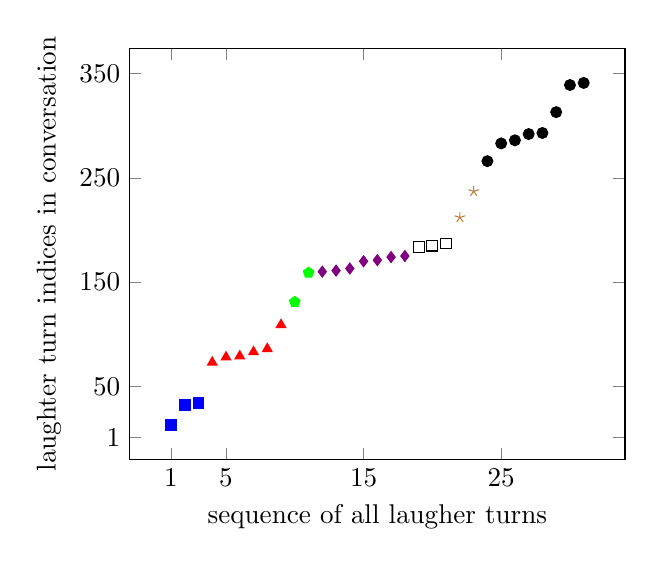
\begin{tikzpicture} [scale=.98]
\begin{axis}[
    xtick={1,5,15,25,35},
    ytick={1,50,150, 250,350},
    xlabel={sequence of all laugher turns},
    ylabel={laughter turn indices in conversation}]
\addplot[
    scatter,
    only marks,
    point meta=explicit symbolic,
    scatter/classes={
      a={mark=square*,blue},%
      b={mark=triangle*,red},%
      c={mark=pentagon*,green},%
      d={mark=diamond*,violet},%
      e={mark=square,black},%
      f={mark=star,brown},%
      g={mark=o,draw=black}},
]
table[meta=label] {
x	y	label
1	13	a
2	32	a
3	34	a
4	73	b
5	78	b
6	79	b
7	83	b
8	86	b
9	109	b
10	131	c
11	159	c
12	160	d
13	161	d
14	163	d
15	170	d
16	171	d
17	174	d
18	175	d
19	184	e
20	185	e
21	187	e
22	212	f
23	237	f
24	266	h
25	283	h
26	286	h
27	292	h
28	293	h
29	313	h
30	339	h
31	341	h
};
%\addplot[
%    scatter,
%    %only marks,
%    point meta=explicit symbolic,
%    scatter/classes={
%      a={mark=square*,blue},%
%      b={mark=triangle*,red},%
%      c={mark=pentagon*,green},%
%      d={mark=diamond*,violet},%
%      e={mark=square,black},%
%      f={mark=star,brown},%
%      g={mark=o,draw=black}},
%]
%table[meta=label] {
%x	y	label
%1	39	a
%2	65	b
%3	129	c
%4	203	d
%5	257	e
%6	345	f
%7	394	g
%};

\end{axis}
\end{tikzpicture}
%\begin{tikzpicture}[scale=.7]
%  \begin{axis}
%    \addplot+[red]
%      coordinates
%        {(1,13)(2,32)(3,34)
%(4,73)(5,78)(6,79)(7,83)
%(8,86)(9,109)
%(10,131)(11,159)(12,160)(13,161)(14,163)
%(15,170)(16,171)(17,174)(18,175)
%(19,184)(20,185)(21,187)
%(22,212)(23,237)(24,266)
%(25,283)(26,286)
%(27,292)(28,293)
%(29,313)
%(30,339)(31,341)};
%  \end{axis}
%\end{tikzpicture}
\caption{\footnotesize The scatterplot of $Bmr026$ conversation with laughter indices vs. number sequences of all laughter occurrences. The different symbols \& colors denote the shared laughter cluster (for e.g. the first cluster of shared laughter is denoted by $3$ blue cubes within first $50$ turn occurrences).}\label{fig:eg}
\end{figure}
\end{center}

We present our results in the Table \ref{tab:res}. The first row and the fourth row present the baseline performances where we used the \emph{BayesTopic} and \emph{BestCluster} algorithm. The second and third rows present our proposed clustering based approaches, \emph{OptimAggloCluster} refers to the approach of segmentation using agglomerative clustering, then optimized with fixed boundary clumping and \emph{OptimKMedoidCluster} refers to the performances of iteratively optimized of the $K$-medoids clustered segmentation. We present the results with two metrics in two columns. %Our proposed clustering based approach could not perform well in comparison to the BayesTopic approach, but the performance is better compared to the random baseline. 
For all the five cases the $P_k$ measure performances marginally work better than the corresponding $WD$ measure performances. Between the two baselines, the \emph{BayesTopic} was harder to overcome. Between two standalone cluster-based approaches (second and third rows of Table \ref{tab:res}) \emph{OptimKMedoidCluster} performs better than the \emph{OptimAggloCluster} approach. The \emph{BestCluster}, which is our second baseline, shows better performance than the standalone cluster based approaches but it shows lower performance than the first baseline the \emph{BayesTopic}. The best performance is performed by our proposed hybrid approach \emph{hybridFrameWrk} that beats both of the baselines for both of the $P_k$ and $WD$ measures. 
%The boundary clumping optimization works well for $WD$ improving the result far better than the basic cluster based approach, because $WD$ metric works better with lesser number of segments than that of $P_k$. We see that the proposed methods works better than a random segmentation. Although the proposed approach poorly performs in comparison to the state-of-the-art segmentation method, the proposed technique uses only a single piece of information in comparison to the existing rich system. 
It is possible to use this method without any change for a range of conversational applications like hybrid, online, multilingual and low resource language systems.

\begin{table}
\begin{center}
\small{
\begin{tabular}{l*{6}{c}r}
\hline \hline
Algorithm  & $P_k$ & $WD$  \\
\hline \hline
BayesTopic \cite{eisenstein-08} & 0.239 & 0.312 \\
%Random  & 0.466 & 0.552 \\
\hline
OptimAggloCluster  & 0.388 & 0.404  \\
OptimKMedoidCluster  & 0.324 & 0.388 \\
BestCluster & 0.317 & 0.379 \\
\hline
hybridFrameWrk (proposed) & 0.190 & 0.248 \\
\hline
\end{tabular}
}
\end{center}
\vspace*{-\baselineskip}
\caption{The baseline and proposed approach results}\label{tab:res}
\end{table}


We observe from Table \ref{tab:indvres} that the hybrid segmentation technique also effective for the individual conversation, more than 90\% of time the performance is improved by the hybrid framework compared to the standalone performances. We notice from the same Table \ref{tab:indvres} that among all the nineteen conversations the conversations $Bmr007$ and $Bmr008$, the proposed hybrid algorithm does not perform better than the \emph{BayesTopic} algorithm, for both the metrics $P_k$ and $WD$. Still the performances are comparable to the best performances in each of these two cases. %We present the results from the hybrid framework for each of the conversations used in this work in the Table \ref{tab:indvres}. 
In the same table we also compute the means and the standard deviation of all the measures in total. We observe that comparatively the standard deviation of the window difference ($WD$) of the \emph{BayesTopic} approach is higher than that of other approaches, whereas the $P_k$ of the same approach is marginally higher than the other values of the two rest approaches.

\begin{table}[htbp]
  \centering
  \resizebox{\columnwidth}{!}{
  \small{
    \begin{tabular}{rcccccc}
    \hline
    \textbf{ICSI ID } & \multicolumn{2}{c}{\textbf{BayesTopic}} & \multicolumn{2}{c}{\textbf{BestCluster}} & \multicolumn{2}{c}{\textbf{Hybrid}} \\
   \hline
    \hline
     & P\_k & WD & P\_k & WD & P\_k & WD \\
    \hline
    Bmr001 & 0.322 & 0.431 & 0.312 & 0.421 & 0.216 & 0.325 \\
    Bmr002 & 0.243 & 0.301 & 0.351 & 0.402 & 0.244 & 0.295 \\
    Bmr005 & 0.289 & 0.374 & 0.296 & 0.381 & 0.186 & 0.271 \\
    Bmr007 & 0.159 & 0.229 & 0.398 & 0.467 & 0.174 & 0.244 \\
    Bmr008 & 0.065 & 0.076 & 0.3 & 0.31 & 0.077 & 0.088 \\
    Bmr009 & 0.299 & 0.426 & 0.325 & 0.342 & 0.247 & 0.265 \\
    Bmr010 & 0.265 & 0.292 & 0.359 & 0.387 & 0.236 & 0.266 \\
    Bmr011 & 0.269 & 0.296 & 0.373 & 0.39 & 0.261 & 0.264 \\
    Bmr012 & 0.258 & 0.475 & 0.175 & 0.379 & 0.125 & 0.329 \\
    Bmr013 & 0.247 & 0.285 & 0.161 & 0.225 & 0.085 & 0.149 \\
    Bmr014 & 0.175 & 0.253 & 0.297 & 0.393 & 0.166 & 0.244 \\
    Bmr018 & 0.326 & 0.42 & 0.297 & 0.393 & 0.21 & 0.288 \\
    Bmr020 & 0.156 & 0.239 & 0.358 & 0.477 & 0.151 & 0.216 \\
    Bmr022 & 0.025 & 0.121 & 0.331 & 0.342 & 0.112 & 0.123 \\
    Bmr024 & 0.349 & 0.458 & 0.313 & 0.407 & 0.204 & 0.258 \\
    Bmr025 & 0.253 & 0.328 & 0.28 & 0.298 & 0.266 & 0.315 \\
    Bmr026 & 0.231 & 0.286 & 0.239 & 0.294 & 0.096 & 0.151 \\
    Bmr027 & 0.295 & 0.317 & 0.436 & 0.452 & 0.292 & 0.294 \\
    Bmr029 & 0.332 & 0.332 & 0.432 & 0.432 & 0.259 & 0.336 \\
     \hline
    \textbf{Mean} & \textbf{0.239} & \textbf{0.312} & \textbf{0.317} & \textbf{0.379} & \textbf{0.19} & \textbf{0.248} \\
    \hline
    \textbf{StdDev} & \textbf{0.088} & \textbf{0.106} & \textbf{0.064} & \textbf{0.064} & \textbf{0.063} & \textbf{0.072} \\
    \hline\hline
    \end{tabular}%
    }}
 \caption{BayesTopic, BestCluster and Hybrid Approach Individual Conversation Analysis Results}\label{tab:indvres}%
\end{table}%

We run the significance testing on lexical cohesion based bayesian approach for text segmentation versus the proposed hybrid framework based on human laugh occurrences in a conversation, we find that the improvement of the performance is significant at the $95\%$ significance level.

We present the number of segments used for the best results for the individual conversations for two stand-alone and hybrid approaches in the Table \ref{tab:segres}. We perform Spearman's $\rho$ correlation test on each pairwise columns. We find that there is least ($\rho=0.10$) correlation between the \emph{BayesTopic} and \emph{BestCluster} number of segment distribution, on the other hand there is more ($\rho=0.46$) correlation between the \emph{BestCluster} and Hybrid approach the number of segment distribution, whereas the segments between the \emph{BayesTopic} and Hybrid approach are also not well-correlated ($\rho=0.26$). We also notice from the Table \ref{tab:segres} that there is no visible correlation between time of running the meeting and the number of discourse-topic segments of conversation. So in case a meeting runs much longer than the others, it does not necessarily mean that there are many local discourse or many topics to discuss. It is an interesting observation in the Table \ref{tab:segres} that for the conversation $Bmr009$ the hybrid algorithm detects only one segment for the best performance. We observe from the $Bmr009$ transcript that the participants tried to make the meeting short with two discussion-topics namely, signal processing and transcription issues, then the individual digit recording started.  

\begin{table}[h!]
\centering
\resizebox{\columnwidth}{!}{
 \begin{tabular}{||c c c c c||} 
 \hline
 ICSI ID & Time(min) & BayesTopic & BestCluster & Hybrid \\ [0.5ex] 
 \hline\hline
 Bmr001 & 36 & 7 & 2 & 4 \\ 
 Bmr002 & 46 & 7 & 4 & 4 \\
 Bmr005 & 71 & 5 & 8 & 5 \\
 Bmr007 & 60 & 4 & 8 & 2 \\
 Bmr008 & 68 & 3 & 5 & 2 \\ 
 Bmr009 & 50 & 7 & 4 & 1 \\
 Bmr010 & 54 & 5 & 6 & 9 \\
 Bmr011 & 67 & 5 & 8 & 5 \\
 Bmr012 & 42 & 6 & 7 & 5 \\
 Bmr013 & 48 & 5 & 7 & 5 \\
 Bmr014 & 50 & 4 & 4 & 4 \\
 Bmr018 & 57 & 5 & 8 & 8 \\
 Bmr021 & 37 & 6 & 9 & 5 \\
 Bmr022 & 50 & 7 & 7 & 3 \\
 Bmr024 & 52 & 9 & 12 & 6 \\
 Bmr025 & 33 & 7 & 5 & 8 \\
 Bmr026 & 45 & 5 & 4 & 4 \\
 Bmr027 & 49 & 5 & 5 & 3 \\
 Bmr029 & 43 & 3 & 2 & 3 \\ [1ex] 
 \hline
 \end{tabular}
 }
 \caption{Number of segments used for BayesTopic, BestCluster and Hybrid Approach for the Best Results (including the time for each of the meetings)}\label{tab:segres}%
\end{table}

Both of the box-plots in the Figure \ref{fig:3boxplot} show significant improvement of the performance of the Hybrid approach over the stand-alone approaches. We observe skewness of \emph{BestCluster} performance with the $P_k$ metrics; on the other hand the \emph{BayesTopic} performance is skewed for $WD$ metrics.  The inter-quantile ranges of the \emph{BayesTopic} performance are longer than the other two approaches, for both of the metrics. We also observe the existence of outliers in the case of \emph{BestCluster} performance for both of the box-plots, whereas we find one outlier data for hybrid approach during the $WD$ box-plot comparison.

\begin{figure}%
    \centering
    \subfloat[$P_k$ Comparison]{{\includegraphics[width=6.5cm]{bsbchybpk.jpg} }}%
    \qquad
    \subfloat[$WD$ Comparison]{{\includegraphics[width=6.5cm]{bsbchybwd.jpg} }}%
    \caption{Boxplot Comparison: BayesTopic vs. BestCluster vs. Hybrid Approaces}%
    \label{fig:3boxplot}%

\end{figure}

In addition, we also tested the modality of the distribution of the $P_k$ and $WD$ for set of partitions of each conversation. We plot the log-normal plot of cumulative values each of of $P_k$ and $WD$ against the time scale, we get a straight line plot from each of the used meeting conversation, which proves the uni-modality of each of the conversation for both of the evaluation metrics. 

%\textit{Interaction between Topic Structure \& Discourse Relational Structure.} 
\subsubsection{Interaction between Topic Structure \& Discourse Relational Structure} We separately parse each of the topic segment of a document through PDTB-styled discourse connective based parser \cite{lin-12} and we collect in-topic keywords. We use a method of collecting all terms on the basis of term-frequency-inverse-document-frequency, then we consider the highly frequent terms using an overlapping 3-turn-windows over the whole segment; we notice patterns that 1. the in-topic keyword density of the topic structure is higher before the commencement of discourse relations and 2. there is a tendency that the explicit connectives do not occur at the beginning of the topic segment. So the fine-grained topics are subjected by the discourse relations. The discourse relations are satisfied if the topic structure constraints are fulfilled. This gives an indication of influence of discourse connectives to link up topic structures together, which helps the global level meaning construction from the local level meanings and also it facilitates disambiguation. Evidences from $Bmr026$ and $Bmr012$ documents are used for this short study. %We found more evidences in $Bmr026$ and $Bmr012$, than in $Bmr002$.

 %Baseline
 \section{Conclusion}\label{sec:concl}
%Human laugh occurrences or laughter possess an important role in human conversation comprehension. There may exist a variety of the laughter: among all of these the shared laughter is studied to be related to the topic change in the conversation, though the vice-versa is not necessarily true, i.e. topic change in a conversation may also happen without a single occurrence of laughter. Thus it enables us to segment a conversational discourse into several conversation segments. The whole process of segmentation is training-free and quick. This algorithm can be used in an incremental learning task. This is perfectly applicable to the real-life scenario of spoken language understanding.
 
In this study, we propose a laughter information based method of hybrid topic structure for the conversational discourse. There are already several successful approaches for topic segmentation; the proposed approach offers a hierarchy of global and local discourse combining coarse and fine-grained segmentation that hybrids paralinguistic and linguistic information from natural discourses. 

The paper has described a novel training-free algorithm that uses only the paralinguistic information, that is the laughter occurrences to segment the whole conversation into several discourse segments in parallel with two clustering techniques: agglomerative and $K$-medoids. These segmentations are further optimized using a boundary clumping algorithm for the agglomerative case and using an iterative for the $K$-medoids case. Then we choose the best performing clustering based approach for each conversation. Finally through an iterative process we hybridize the fine-level segmentation of a third party Bayesian segmentation tool for each of the coarse level segmentation through clustering. Our proposed approach achieves a hybrid topic structure of coherence that out performs the stand-alone approaches. %To our best knowledge no framework is devised till date that uses shared laughter as the anchor points to segment the whole conversational discourse. %This clustering based method is easily portable to any language. 

This frame-work can be applicable to the online scenario of spoken language understanding. %: 1. the laugher occurrences does not need language 2. the unsupervised Bayesian approach can be easily adapted to even a low resource language. It is a training free approach. 
Through the brief study we find that there is an opportunity for an in-depth study of interactions between the topic structure and the other discourse structures, namely discourse relational structure.
\section{Acknowledgement}
This work was primarily done in Idiap Research Institute, Switzerland. The author thanks to Dr. Mathew Magimai Doss and Dr. Afsaneh Asaei for all help.

\bibliographystyle{hacm}
\bibliography{references}



\end{document}
